\section{Conception et réalisation}

\subsection{Partir de l'utilisateur pour arriver au diagramme.}

En premier lieu il nous a semblé intéressant de s'imaginer le comportement d'un utilisateur devant le programme fini. Ainsi, au fil des actions du personnage virtuel,
l'allure globale du projet se détaille.  

Le schéma d'utilisation classique part d'une importation d'un ensemble de dossiers ou fichiers de type Open Document Text ( abrégé ODT par la suite ), l'extraction d'un fichier contenant les données à analyser, l'analyse, et le stockage, ces trois dernières étapes étant totalement transparentes pour l'utilisateur.
Ensuite vient la recherche. L'utilisateur doit pouvoir entrer un ou plusieurs mots et avoir en retour une liste triée par pertinence des documents ODT les plus pertinents. 

L'étape suivante consiste à abstraire le problème en passant par un diagramme de classes UML. Après différentes discussions, le diagramme approuvé par notre groupe est celui-ci.
 \begin{figure}[!ht]
	\center
	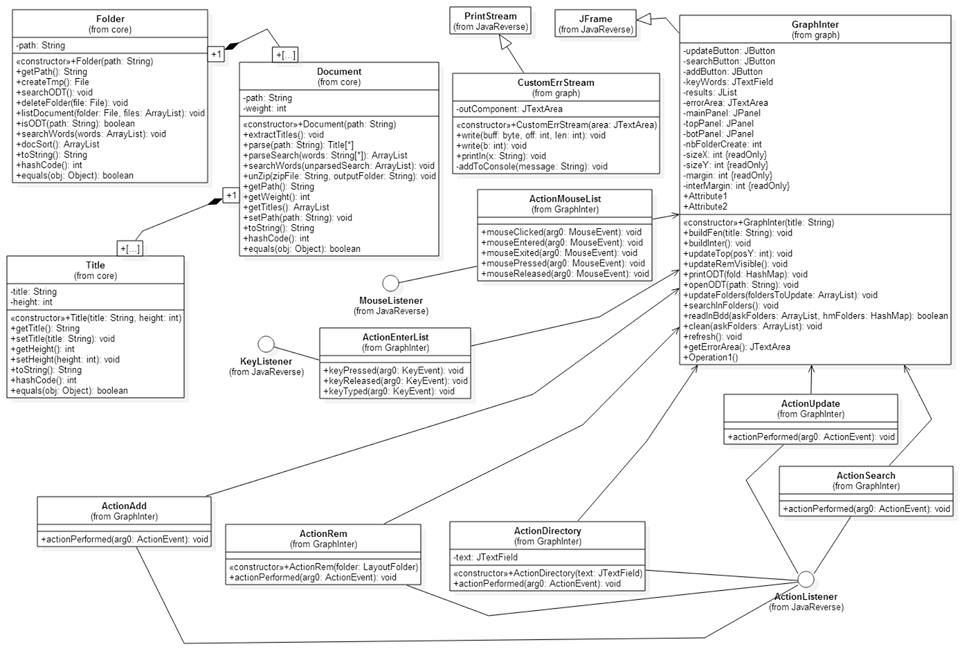
\includegraphics[width=\textwidth]{./images/uml.jpg}
	\caption{\href{http://uinelj.eu/misc/yolODT/uml.jpg}{Voir l'UML en plus grand}}
\end{figure}

\subsection{Du diagramme au code.}

Au vu de la taille du projet, la réalisation a nécessité un partage des tâches. 
Afin d'avoir une gestion du projet efficace, simple et sûre, un dépôt git\footnote{git est un logiciel de gestion de versions.} a été créé.
Ainsi, chaque modification du code est expliquée, enregistrée, et réversible en cas de problème. 

Concernant le partage des tâches suscité, Bastien s'est plus occupé des aspects d'entrée/sortie, de gestion des fichiers et de l'interface graphique, tandis que Julien
s'est focalisé sur l'extraction, l'analyse (parsage XML) et l'interface en ligne de commande. 

Le partage n'a cependant pas été hermétique : Nous nous avous mutuellement relu notre code et suggéré des améliorations. Un exemple est la gestion de la recherche. Initalement réalisée par la méthode searchWords écrite par Bastien, Julien l'a modifié légèrement et y a adjoint la méthode parseSearch, afin de proposer des possibilités de recherche plus étendues.
% On peut mettre des mots en \emph{italique}, 
% en \textsc{petites Majuscules} ou 
% en \texttt{largeur fixe (machine à écrire)}.

% Voici un deuxième paragraphe avec une formule mathématique simple : $e = mc^2$.

% Un troisième avec des \og guillemet français \fg{}.

% \subsubsection{Écrire en anglais}

% \foreignlanguage{english}{Do you speak French? Does anybody here speak french?}


% \subsection{Lites}

% \begin{itemize}
% \item Liste classique ;
% \item un élément ;
% \item et un autre élément.
% \end{itemize}
% \vspace{\parskip} % espace entre paragraphes

% \begin{enumerate}
% \item Une liste numéroté
% \item deux
% \item trois
% \end{enumerate}
% \vspace{\parskip}

% \begin{description}
% \item[Description] C'est bien pour des définitions.
% \item[Deux] Ou pour faire un liste spéciale.
% \end{description}
% \vspace{\parskip}


% \subsection{Références}

% Voici une référence à l'image de la figure \ref{bloghiko} page \pageref{bloghiko} et une autre vers la partie \ref{p2} page \pageref{p2}.

% On peut citer un livre\,\up{\cite{lpp}} et on précise les détails à la fin du rapport dans la partie références.


% \subsection{Note de bas de page}

% Voici une note\,\footnote{Texte de bas de page} de bas de page.
% Une deuxième\,\footnotemark{} déclarée différemment.
% La même note\,\footnotemark[\value{footnote}].

% \footnotetext{Il a deux références vers cette note}


% \subsection{Figure}

% \begin{figure}[!ht]
%     \center
%     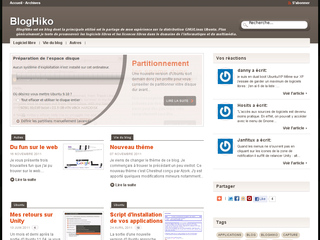
\includegraphics[width=0.5\textwidth]{./images/bloghiko.jpg}
%     \caption{BlogHiko | 50\% de la largeur de la page}
% \end{figure}


